\chapter{IMPLEMENTATION DETAILS}

The implementation of the system to convert hand-drawn circuit diagrams into simulation-ready netlists and digital schematics follows a modular approach, aligning with the pipeline described in the architecture and methodology. Some of the methodologies explained in the previous section, that have been implemented are explained in this section.

\section{Dataset Manipulation and Preprocessing}

\subsection{Conversion of Annotation Formats}

To accommodate the multiple models in the pipeline (YOLOv7 for component detection and \gls{ocr} for value extraction), annotation files provided in the \gls{cghd} dataset in Pascal VOC (XML) format were converted into compatible formats. Likewise, for EasyOCR-inspired custom-trained \gls{ocr}, all text-sections needed to be cropped out from the image with corresponding labels (ground truth) and then fed to the fine-tuned model.

In Pascal VOC format, the information regarding the circuit and its components are stored in the following format as shown by the example below:

\begin{lstlisting}[language=XML, frame=none, numbers=none, backgroundcolor=, basicstyle=\ttfamily\fontsize{12}{14}\selectfont, label={lst:pascal-voc-example}]
<annotation>
    <folder>images</folder>
    <filename>C1_D1_P2.jpg</filename>
    <path>./drafter_1/images/C1_D1_P2.jpg</path>
    <source>
        <database>CGHD</database>
    </source>
    <size>
        <width>3024</width>
        <height>4032</height>
        <depth>3</depth>
    </size>
    <segmented>0</segmented>
    <object>
        <name>voltage.dc</name>
        <pose>Unspecified</pose>
        <truncated>0</truncated>
        <difficult>0</difficult>
        <bndbox>
            <xmin>327</xmin>
            <ymin>546</ymin>
            <xmax>604</xmax>
            <ymax>838</ymax>
            <rotation>10</rotation>
        </bndbox>
    </object>
</annotation>
\end{lstlisting}

For \gls{yolo}-based detection, XML annotations were converted to \gls{yolo} format (\texttt{.txt}) using a custom \gls{python} script. Each \texttt{.txt} file contains the class index and normalized bounding box coordinates in the format:

\begin{center}
\texttt{<class\_id> <x\_center> <y\_center> <width> <height>}
\end{center}

The pseudocode for the VOC to YOLO annotation conversion is as follows:

\begin{algorithm}
\caption{VOC to YOLO Annotation Conversion}
\label{algo:voc-to-yolo}
\begin{algorithmic}
\Require XML annotation file $X$, class map $C$, image width $W$, image height $H$
\Ensure List of YOLO formatted annotation lines $Y$
\State Parse XML file $X$ into tree structure
\State $Y \leftarrow \emptyset$
\For{all object nodes $o$ in XML root}
    \State $\text{clsname} \leftarrow$ class name of $o$
    \If{$\text{clsname} \notin C$}
        \State \textbf{continue}
    \EndIf
    \State $\text{clsid} \leftarrow C[\text{clsname}]$
    \State Extract bounding box $(x_{\min}, y_{\min}, x_{\max}, y_{\max})$ from $o$
    \State Convert VOC coordinates to normalized YOLO format
    \State $x_{\text{center}} \leftarrow \frac{x_{\min} + x_{\max}}{2W}$
    \State $y_{\text{center}} \leftarrow \frac{y_{\min} + y_{\max}}{2H}$
    \State $w \leftarrow \frac{x_{\max} - x_{\min}}{W}$
    \State $h \leftarrow \frac{y_{\max} - y_{\min}}{H}$
    \State Append formatted string $(x_{\text{center}}, y_{\text{center}}, w, h)$ to $Y$
\EndFor
\State \Return $Y$
\end{algorithmic}
\end{algorithm}

The calculations run for this conversion is as follows:

\begin{equation}
x_{\text{center}} = \frac{327 + 604}{2 \times 3024} = \frac{465.5}{3024} = 0.1539
\label{eq:voc-yolo-x}
\end{equation}

\begin{equation}
y_{\text{center}} = \frac{546 + 838}{2 \times 4032} = \frac{692}{4032} = 0.1716
\label{eq:voc-yolo-y}
\end{equation}

\begin{equation}
w = \frac{604 - 327}{3024} = \frac{277}{3024} = 0.0916
\label{eq:voc-yolo-w}
\end{equation}

\begin{equation}
h = \frac{838 - 546}{4032} = \frac{292}{4032} = 0.0724
\label{eq:voc-yolo-h}
\end{equation}

This gives the information required by \gls{yolo} in the appropriate format. It is convention to save this new annotation file in the same directory as the image.

Likewise, for \gls{ocr} compatibility, the same Pascal VOC annotations were converted to \gls{lmdb} format. \gls{lmdb} is a high-speed key-value store where each key corresponds to an index and each value contains an image-text pair (serialized).

The pseudocode for the conversion of Pascal VOC format to \gls{ocr}-compatible \gls{lmdb} file format is as follows:

\begin{algorithm}
\caption{Image Cropping and LMDB Dataset Creation}
\label{algo:image-crop-lmdb}
\begin{algorithmic}
\Require Input image file $I$, crop coordinates $(y_{\min}, y_{\max}, x_{\min}, x_{\max})$, target size $(W, H)$
\Ensure \gls{lmdb} database containing image-label pairs
\State Load image $I$ into memory
\State Crop image using coordinates $[y_{\min} : y_{\max}, x_{\min} : x_{\max}]$
\State Resize cropped image to size $(W, H)$
\State Convert cropped image to byte representation
\State Convert image array to PIL image
\State Initialize in-memory byte buffer
\State Save image to buffer in JPEG format
\State Extract byte stream from buffer
\State Store image and label in \gls{lmdb}
\State Open \gls{lmdb} environment with predefined map size
\State Begin write transaction
\State Store image bytes with key \texttt{image-00001}
\State Store corresponding label with key \texttt{label-00001}
\State Store total sample count with key \texttt{num-samples}
\State Commit transaction
\State \Return \gls{lmdb} environment
\end{algorithmic}
\end{algorithm}

After this script is run in its entirety, a file in \gls{lmdb} format, as is expected by \gls{ocr}, is received as shown in the example below:

\begin{lstlisting}[frame=none, numbers=none, backgroundcolor=, basicstyle=\ttfamily\fontsize{12}{14}\selectfont, label={lst:lmdb-example}]
Key: b'image-00001'
Value: b'\xff\xd8\xff\xe0\x00\x10JFIF...'

Key: b'label-00001'
Value: b'voltage.dc'

Key: b'num-samples'
Value: b'000001'
\end{lstlisting}

After necessary conversion, the dataset was ready for being plugged into the required models for fine-tuning them. But first, some experimentation was done with different forms of image augmentation techniques.

\subsection{Image Augmentation}

Since the dataset contains handwritten circuit diagrams captured under variable lighting and orientations, several augmentation techniques were applied to improve model generalization including Contrast Enhancement (global) and Adaptive Brightness Adjustment by factors of 0.8 and 1.2. Furthermore, geometric augmentation techniques, like spatial flipping (both horizontally and vertically) and rotation (e.g., $90^\circ$ or random rotation) proved to be unwise operations for this project. For example, if a ``C'' is rotated by $90^\circ$, the ``C'' now resembles a ``U'', and the same applies to flipping (``M'' might look like ``W'', for example). Rather than increasing accuracy, it was realized that using rotation or flipping would simply confuse the model. However, continuous testing with other forms of augmentation will continue in hopes of improving the model.

\subsection{Fine-tuning YOLOv5 and YOLOv7 for Component Detection}

YOLOv5 was initially used for benchmarking, and later upgraded to YOLOv7 for better accuracy and inference speed (comparison shown in the Results section). Training and fine-tuning were done using the \gls{cghd} dataset after converting into \gls{yolo}-compatible format.

The training parameters employed are as follows:

\begin{itemize}
    \item \textbf{Number of classes:} 61
    \item \textbf{Training split:} 70\% training, 10\% validation, 20\% testing
    \item \textbf{Epochs:} 200 (for YOLOv5), 100 (for YOLOv7)
    \item \textbf{Image size:} $416 \times 416$ pixels
    \item \textbf{Batch size:} 16 (for YOLOv5), 32 (for YOLOv7)
    \item \textbf{Optimizer:} \gls{sgd} (Stochastic Gradient Descent)
    \item \textbf{Learning rate:} 0.01 (initial)
    \item \textbf{Augmentations used in training:} Mosaic Augmentation, \gls{hsv} Augmentation, Random rotating/flipping
\end{itemize}

\subsection{Implementation of Text Recognition (OCR)}

To extract textual information such as resistor values, capacitor labels, and other component annotations from the circuit diagrams, a \gls{crnn}-based custom \gls{ocr} model was chosen, trained and implemented. The input image in cropped form (cropped for each text component) was passed through this model after training, which returned the content of each detected text element. The position of said text element, however, was found using bounding boxes from YOLOv7. This allowed us to localize and read numerical values or labels directly from the circuit.

Three different modules, each for feature extraction, sequence modeling, and prediction were trained based on the DTRB framework. Initially, simply fine-tuning \gls{ocr} models like TrOCR and EasyOCR were also attempted; however, these didn't yield usable results, ultimately requiring training from scratch. The training was done for 29 epochs.

\subsection{Line Detection Algorithm Implementation}

The line detection mechanism was engineered to exploit the semantic constraints of circuit diagrams, specifically that wires are predominantly axis-aligned (horizontal or vertical) and connect distinct components. Unlike the Probabilistic Hough Transform (\gls{pht}) which operates purely on pixel gradients, this approach uses the junction points detected by YOLOv7 as anchor nodes to reconstruct the wiring layout geometrically.

First, a pairwise analysis was performed on all junction points identified by the object detection model. The algorithm iterates through every unique pair of junctions to calculate the angle of the vector connecting them. Since hand-drawn circuits contain imperfections, an angular tolerance of $\pm 18^\circ$ was applied to classify connections as either horizontal or vertical. To ensure coordinate consistency across the diagram, the resulting segment coordinates were ``snapped'' to a grid using a 16-pixel quantization.

\begin{algorithm}
\caption{Wire Classification and Alignment}
\label{algo:wire-classification-impl}
\begin{algorithmic}
\Require Set of junctions $J$, angular tolerance $\omega_{\text{tol}} = 18^\circ$, grid size $g = 16$
\Ensure Set of raw wire segments $S$
\State $S \leftarrow \emptyset$
\For{all pairs $(j_a, j_b) \in \text{Combinations}(J, 2)$}
    \State $\Delta x \leftarrow j_b.x - j_a.x$
    \State $\Delta y \leftarrow j_b.y - j_a.y$
    \State $\theta \leftarrow \text{atan2}(\Delta y, \Delta x)$
    \If{$|\theta| \le \omega_{\text{tol}} \lor |\theta - 180^\circ| \le \omega_{\text{tol}}$}
        \State \textbf{Horizontal alignment check}
        \State $y_{\text{avg}} \leftarrow \frac{j_a.y + j_b.y}{2}$
        \State $y_{\text{snap}} \leftarrow \text{Round}\left(\frac{y_{\text{avg}}}{g}\right) \times g$
        \State $S \leftarrow S \cup \{(H, y_{\text{snap}}, \min(j_a.x, j_b.x), \max(j_a.x, j_b.x))\}$
    \ElsIf{$|\theta - 90^\circ| \le \omega_{\text{tol}} \lor |\theta - 270^\circ| \le \omega_{\text{tol}}$}
        \State \textbf{Vertical alignment check}
        \State $x_{\text{avg}} \leftarrow \frac{j_a.x + j_b.x}{2}$
        \State $x_{\text{snap}} \leftarrow \text{Round}\left(\frac{x_{\text{avg}}}{g}\right) \times g$
        \State $S \leftarrow S \cup \{(V, x_{\text{snap}}, \min(j_a.y, j_b.y), \max(j_a.y, j_b.y))\}$
    \EndIf
\EndFor
\State \Return $S$
\end{algorithmic}
\end{algorithm}

A common issue with the pairwise approach is the generation of redundant, overlapping segments for the same wire. For instance, if three junctions lie on a single line, the algorithm produces three separate segments (A-B, B-C, and A-C). To combat this, a collinear segment merging algorithm was implemented.

The segments were first separated by orientation (horizontal/vertical) and sorted by their primary axis. The merging logic then consolidated overlapping or adjacent segments. Crucially, a length-weighted heuristic was used: when merging, the axis coordinate of the longer segment was preserved, ensuring that larger, more reliable strokes dictated the final geometric alignment.

\begin{algorithm}
\caption{Collinear Segment Merging}
\label{algo:segment-merging-impl}
\begin{algorithmic}
\Require List of segments $L$, gap tolerance $\omega$
\Ensure List of merged segments $M$
\State Sort $L$ by primary axis, then by starting coordinate
\State $M \leftarrow \emptyset$
\State $\text{curr} \leftarrow L[0]$
\For{all $\text{next} \in L[1 \ldots N]$}
    \If{$|\text{curr.axis} - \text{next.axis}| \le \omega \land \text{next.start} \le \text{curr.end} + \omega$}
        \State $\text{curr.start} \leftarrow \min(\text{curr.start}, \text{next.start})$
        \State $\text{curr.end} \leftarrow \max(\text{curr.end}, \text{next.end})$
        \If{$\text{Length}(\text{next}) > \text{Length}(\text{curr})$}
            \State \textbf{Preserve axis of the longer segment}
            \State $\text{curr.axis} \leftarrow \text{next.axis}$
        \EndIf
    \Else
        \State $M \leftarrow M \cup \{\text{curr}\}$
        \State $\text{curr} \leftarrow \text{next}$
    \EndIf
\EndFor
\State $M \leftarrow M \cup \{\text{curr}\}$
\State \Return $M$
\end{algorithmic}
\end{algorithm}

The wire–component intersection detection algorithm identifies precise connection points between detected wire segments and component bounding boxes. Component regions are first extracted from YOLOv7 annotations and converted into pixel coordinates. Each horizontal and vertical wire is then tested for geometric intersection with the edges of every component box. The resulting intersection points are used to accurately map circuit connectivity and are optionally visualized for verification in the frontend.

\begin{algorithm}
\caption{Wire–Component Intersection Detection}
\label{algo:wire-component-intersection-impl}
\begin{algorithmic}
\Require Wire segments $W$, \gls{yolo} label file $L$, image width $I_w$, image height $I_h$
\Ensure Set of intersection points $P$
\State Parse label file $L$
\State Convert normalized bounding boxes to pixel coordinates
\State Discard non-component classes
\State Store component boxes $B$
\State \textbf{Detect intersections between wires and components}
\State $P \leftarrow \emptyset$
\For{all wire $w \in W$}
    \For{all box $b \in B$}
        \If{$w$ is horizontal and crosses left or right edge of $b$}
            \State Add intersection point to $P$
        \ElsIf{$w$ is vertical and crosses top or bottom edge of $b$}
            \State Add intersection point to $P$
        \EndIf
    \EndFor
\EndFor
\State Draw wires, component boxes, and intersection points on image
\State Save output visualization
\State \Return $P$
\end{algorithmic}
\end{algorithm}

\section{Frontend and Backend Implementation}

The frontend system has been realized using React.js, Chart.js and relevant packages like react-draggable and KiCad Symbol Library. Likewise, the backend of the \gls{circuitron} system exposes a \gls{restful} \gls{api} that manages the complete lifecycle of circuit simulations. The \gls{api} provides endpoints for submitting \gls{spice} netlists, validating circuit syntax, and executing simulations using different analysis modes such as transient, \gls{ac}, and \gls{dc} analysis. 

Each simulation request is assigned a unique identifier, enabling asynchronous execution and progress tracking through dedicated status endpoints. The \gls{api} also supports retrieval of detailed simulation results, including time-domain voltage and current data, as well as administrative operations such as stopping running simulations, listing historical simulations, and deleting completed or failed runs. Standard \gls{http} status codes and structured \gls{json} responses are used throughout the \gls{api} to ensure consistency, robust error handling, and seamless integration with the frontend application.

% \subsection{API Endpoints}

% The following table summarizes the key endpoints exposed by the backend \gls{api}:

% \begin{table}[H]
%     \centering
%     \caption{Endpoints Used in the Web Application}
%     \label{table:api-endpoints}
%     \footnotesize
%     \setlength{\tabcolsep}{4pt}
%     \begin{tabular}{|p{1.2cm}|p{4cm}|p{4cm}|}
%         \hline
%         \textbf{HTTP Method} & \textbf{Endpoint} & \textbf{Functionality} \\
%         \hline
%         GET & /api/v1/ & Returns basic API information and available documentation links (health check) \\
%         \hline
%         POST & /api/v1/simulation/simulate & Submits a SPICE netlist and initiates a circuit simulation \\
%         \hline
%         POST & /api/v1/simulation/validate & Validates the syntax and structure of a SPICE netlist without running simulation \\
%         \hline
%         GET & /api/v1/simulation/\{simulation\_id\}/status & Retrieves the current status and progress of a specific simulation \\
%         \hline
%         GET & /api/v1/simulation/\{simulation\_id\}/results & Fetches completed simulation results including voltage, current, and time data \\
%         \hline
%         POST & /api/v1/simulation/\{simulation\_id\}/stop & Stops a currently running simulation \\
%         \hline
%         GET & /api/v1/simulation/ & Lists all simulations with their statuses and creation timestamps \\
%         \hline
%         DELETE & /api/v1/simulation/\{simulation\_id\} & Deletes a simulation and its associated results \\
%         \hline
%         GET & /api/v1/docs & Provides interactive Swagger UI for API exploration \\
%         \hline
%         GET & /api/v1/redoc & Provides ReDoc-based API documentation \\
%         \hline
%         GET & /api/v1/openapi.json & Returns OpenAPI specification in JSON format \\
%         \hline
%     \end{tabular}
% \end{table}




\subsection{Frontend-Backend Interaction}

\begin{figure}[H]
    \centering
    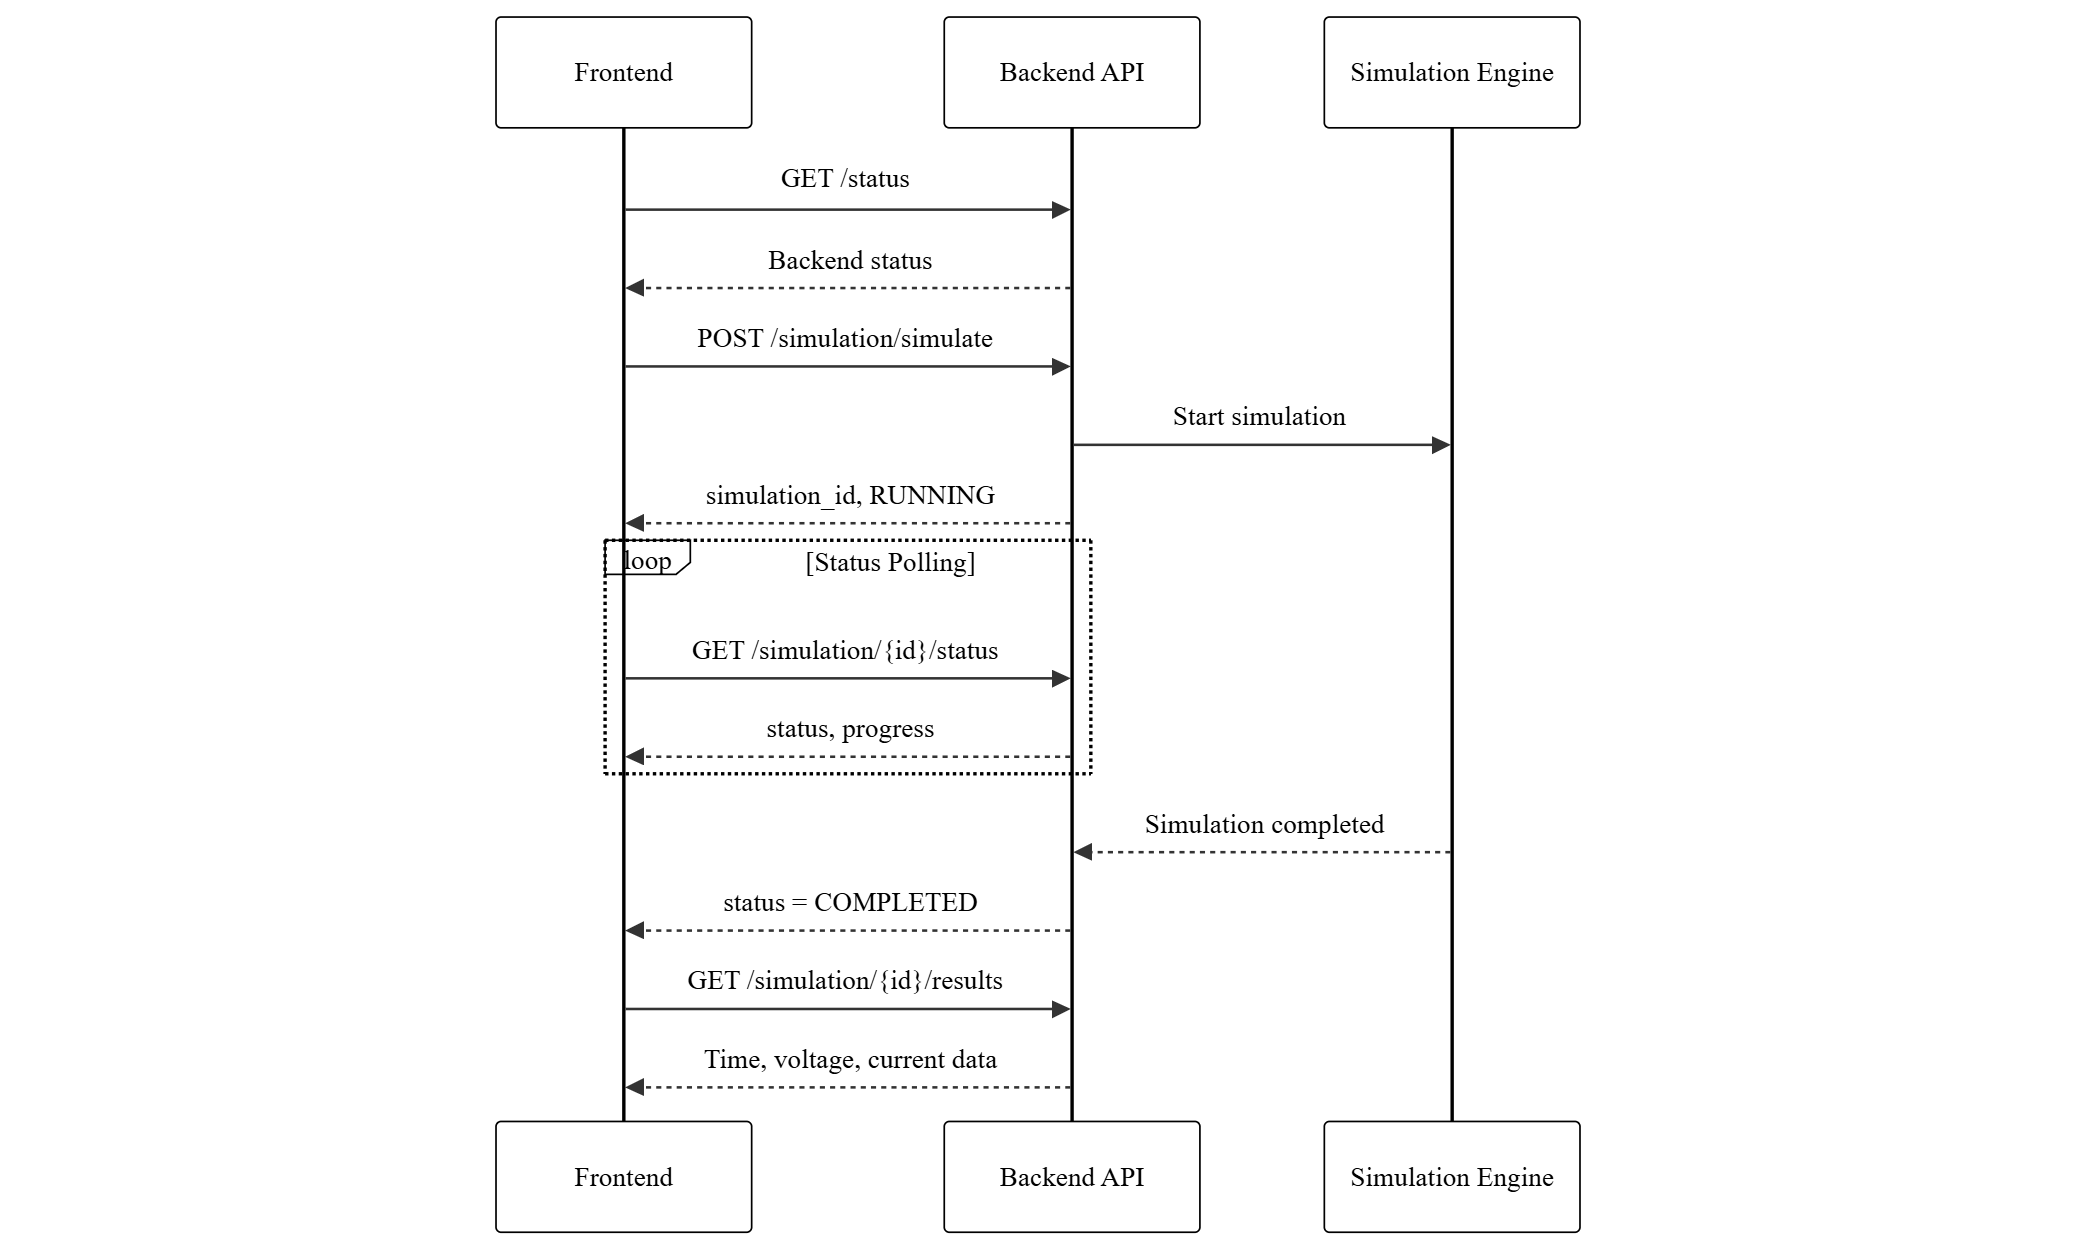
\includegraphics[width=\textwidth]{src/images/figures/backend_req_res.png}    \caption{Interaction Diagram for the Web Application}
    \label{fig:webapp-interaction}
\end{figure}

The frontend communicates with the backend through \gls{http} requests to the documented endpoints. User inputs from the editable circuit schematic are converted into \gls{spice} netlists and submitted to the simulation endpoint. The frontend periodically polls the status endpoint to track simulation progress, and upon completion, retrieves and visualizes the results using Chart.js for graph generation and React components for interactive display.

\section{Circuit Simulation using PySpice}

\gls{pyspice} is a \gls{python} interface to \gls{ngspice} (an open-source simulation engine) that takes in the netlist of the circuit and returns the data required to visualize graphs related to the circuit. The \gls{pyspice} integration allows the backend to programmatically define circuits, run simulations, and extract result data in a structured format suitable for visualization and analysis.

\subsection{Netlist to Simulation Results Conversion}

The process of converting a circuit netlist to simulation results involves several key steps: parsing the netlist, initializing the simulation environment, configuring analysis parameters, executing the simulation, and extracting the resulting voltage and current data in a format compatible with the frontend visualization system.

\begin{algorithm}
\caption{\gls{rc} Circuit Transient Simulation and Data Export}
\label{algo:rc-transient-simulation}
\begin{algorithmic}
\Require Supply voltage $V_s$, resistance $R$, capacitance $C$, simulation step $\Delta t$, simulation duration $T$
\Ensure \gls{csv} file containing transient voltage response
\State Initialize \gls{spice} circuit named \textit{RC Charging Circuit}
\State Enable logging for simulation diagnostics
\State \textbf{Define circuit components}
\State Add \gls{dc} voltage source of magnitude $V_s$ between input node and ground
\State Connect resistor $R$ between input node and node $n1$
\State Connect capacitor $C$ between node $n1$ and ground
\State Initialize simulator with nominal temperature
\State Perform transient analysis with step size $\Delta t$ up to time $T$
\State Extract time vector from transient analysis
\State Extract voltage waveform at node $n1$
\State Create data table mapping time to voltage
\State Export data table to \gls{csv} file
\State \Return Generated \gls{csv} file
\end{algorithmic}
\end{algorithm}

